%\bigskip
%\hrule
%\smallskip
%\hfill Edited by Takayoshi Shoudai on 2024-05-18 (2nd version), 2024-11-18 (3rd version).

\subsection{$D = \{ ya, bc, dy \}$}\label{subsec:d3}

\newcommand{\TheConditionA}{$b \not\in \{a,d\} \mbox{~and~} c \not\in \{a,d\}$}
\newcommand{\TheConditionB}{$b = a,~b \not= d, \mbox{~and~} c \not\in \{a,d\}$}
\newcommand{\TheConditionBsub}{$c \not\in \{a,d\}$}
\newcommand{\TheConditionC}{$b \not\in \{a, d\},~c \not= a, \mbox{~and~} c = d$}

\begin{lem}\label{lem:addpart}
  Let $\Sigma$ be an alphabet with $\sharp\Sigma \ge 3$ and $p,~q$ regular patterns on $\Sigma\cup X$.
  Let $D$ be the following set of regular patterns on $\Sigma\cup X$, where $y$ is a variable symbol in $X$ that does not appear in $p$ and $q$:
  \begin{enumerate}
  \item[] $D = \{ ya, bc, dy \}$ (\TheConditionA).
  \end{enumerate}
  Then, if $p \{ x := r \} \preceq q$ for all $r \in D$, then $p \{ x := xy \} \preceq q$:
\end{lem}

  \begin{proof}
  %If no variable symbol appears in $p$, the statement holds trivially.
  %Thus, for a variable symbol $x\in X$, let $p=p_{1}xp_{2}$, where each $p_{i}$ ($i=1,2$) is either an empty symbol or a regular pattern on $\Sigma\cup X$.
  We assume that $p \{ x := xy \} \not \preceq q$ in order to derive a contradiction.

  Since $p \{ x := r \} \preceq q$ for all $r \in D$, there are three strings of length $2$ in $q$ corresponding to $ya, bc, dy$.
  Note that the three strings may appear with partial overlaps.
  The symbols in $D$ correspond to either a variable or a constant symbol in $q$.
  Let $y_{1}, y_{2}, y_{3}$ be variable symbols appearing in $q$.
  The strings $ya$ and $dy$ must correspond to the strings $y_{1}a$ and $dy_{2}$ in $q$, respectively.
  There are three possible strings in $q$ that correspond to $bc$ in $p\{x:=bc\}$, as follows:
  \begin{center}
    \begin{tabular}{cccccc}
      \textrm{(a)} & $bc$, & \textrm{(b)} & $y_{3}c$, & \textrm{(c)} & $by_{3}$.
    \end{tabular}
  \end{center}

  Suppose that there exists (b) $y_{3}c$ in $q$ that corresponds to $bc$ in $p\{x:=bc\}$, i.e., there exist $q_{1}$ and $q_{2}$, each of which is the empty string or a regular pattern on $\Sigma\cup X$, such that:
  \begin{enumerate}
  \item[(1)] $p_{1}bcp_{2} \preceq q_{1}y_{3}cq_{2}$, 
  \item[(2)] either $p_{1} \preceq q_{1}$ or $p_{1} \preceq q_{1}y_{3}^{\prime}$ for some variable symbol $y_{3}^{\prime}\in X$, and
  \item[(3)] $p_{2} \preceq q_{2}$.
  \end{enumerate}
  In this case, it is straightforward to see that $p\{x:=yc\} = p_{1}ycp_{2} \preceq q_{1}y_{3}cq_{2}$ also holds.
  Thus, both $p\{x:=ya\}\preceq q$ and $p\{x:=yc\}\preceq q$ hold. Since $c\not= a$, by (ii) in Lemma \ref{lem:twovariables}, $p\{x:=xy\}\preceq q$ also holds. This contradicts the assumption.
  Similarly, the case (c) leads to a contradiction by (i) in Lemma \ref{lem:twovariables}.
  Therefore, in the following, we consider only case (a).

  Since $p \{ x := xy \} \not \preceq q$ and the condition \TheConditionA\ hold, the regular pattern $q$ can be expressed in one of the following forms: Let $y_{1}, y_{2}$ be distinct variable symbols in $X$ and $q_{1}, q_{2}, w, w^{\prime}$ be either the empty string or a regular pattern on $\Sigma\cup X$.
  \begin{enumerate}
  \item[(a1)] $q=q_{1}AwBw^{\prime}Cq_{2}$, where $\{ A,B,C \} = \{ y_{1}a,bc,dy_{2} \}$,
  \item[(a2)] $q=q_{1}AwBq_{2}$, where $\{ A,B \} = \{ dy_{1}a,bc \}$,
  \item[(a3)] $q=q_{1}AwBq_{2}$, where $\{ A,B \} = \{ y_{1}ay_{2},bc \}$ ($a = d$).
  \end{enumerate}
  
  First, we consider case (a1).

  \smallskip

  \noindent
  \textit{Claim} 1. $B \not\in \{y_{1}a, dy_{2}\}$.

  \smallskip
  \noindent
  \textit{Proof of Claim} 1.
  Suppose that $(A, B, C) = (dy_{2}, y_{1}a, bc)$. The following conditions must be satisfied: For $y_{1}^{\prime},y_{2}^{\prime}\in X$, 
  \begin{align*}
    \textrm{(1)}~& p_{1} \preceq q_{1}, & \textrm{(1')}~& p_{2} \preceq wy_{1}aw^{\prime}bcq_{2}\mbox{ or} \\
    & & & p_{2} \preceq y_{2}^{\prime}wy_{1}aw^{\prime}bcq_{2},\\
    \textrm{(2)}~& p_{1} \preceq q_{1}dy_{2}w\mbox{ or}  & \textrm{(2')}~& p_{2} \preceq w^{\prime}bcq_{2},\\
    & p_{1} \preceq q_{1}dy_{2}wy_{1}^{\prime}, & & \\
    \textrm{(3)}~& p_{1} \preceq q_{1}dy_{2}wy_{1}aw^{\prime}, & \textrm{(3')}~& p_{2} \preceq q_{2}.
  \end{align*}
  When $p_{2} \preceq wy_{1}aw^{\prime}bcq_{2}$ in (1') holds, let $q^{\prime}_{1}=q_{1}dy_{2},~q^{\prime}_{2}=wy_{1}aw^{\prime},~q^{\prime}_{3}=bcq_{2}$.
  Since $p_{1} \preceq q_{1}dy_{2}wy_{1}aw^{\prime}$ holds from (3), both $p_{1} \preceq q^{\prime}_{1}q^{\prime}_{2}$ and $p_{2} \preceq q^{\prime}_{2}q^{\prime}_{3}$ hold, and $q_{2}^{\prime}$ contains a variable symbol.
  %
  When $p_{2} \preceq y_{2}^{\prime}wy_{1}aw^{\prime}bcq_{2}$ in (1') holds, let $q^{\prime}_{1}=q_{1}d,~q^{\prime}_{2}=y_{2}wy_{1}aw^{\prime},~q^{\prime}_{3}=bcq_{2}$.
  Since $p_{1} \preceq q_{1}dy_{2}wy_{1}aw^{\prime}$ holds from (3), both $p_{1} \preceq q^{\prime}_{1}q^{\prime}_{2}$ and $p_{2} \preceq q^{\prime}_{2}q^{\prime}_{3}$ hold, and $q_{2}^{\prime}$ contains a variable symbol.
  In both cases, by Theorem~\ref{Sato1:Lemma9}, $p \preceq q$ holds.
  This contradicts the assumption that $p \{ x := xy \} \not \preceq q$.

  Similarly, we can show that any case where $(A, B, C) = (y_{1}a, dy_{2}, bc)$, $(bc, y_{1}a, dy_{2})$, or $(bc, dy_{2}, y_{1}a)$ also contradicts the assumption.
  %
  Therefore, we have $B \not\in \{y_{1}a, dy_{2}\}$. (\textit{End of Proof of Claim})

  \smallskip

  \noindent
  \textit{Claim} 2. $(A, B, C) = (y_{1}a, bc, dy_{2})$.

  \smallskip
  \noindent
  \textit{Proof of Claim} 2.
  From \textit{Claim} 1, we have $B=bc$. Suppose that $(A, B, C) = (dy_{2}, bc, y_{1}a)$, i.e., $q = q_{1}dy_{2}wbcw^{\prime}y_{1}aq_{2} $ holds.
  Then, the following conditions must be satisfied: For $y_{1}^{\prime},y_{2}^{\prime}\in X$,
  \begin{align*}
  \textrm{(1)}~& p_{1} \preceq q_{1}, & \textrm{(1')}~& p_{2} \preceq wbcw^{\prime}y_{1}aq_{2}\mbox{ or}\\
  & & & p_{2} \preceq y_{2}^{\prime}wbcw^{\prime}y_{1}aq_{2},\\
  \textrm{(2)}~& p_{1} \preceq q_{1}dy_{2}w, & \textrm{(2')}~& p_{2} \preceq w^{\prime}y_{1}aq_{2}, \\
  \textrm{(3)}~& p_{1} \preceq q_{1}dy_{2}wbcw^{\prime}\mbox{ or} & \textrm{(3')}~& p_{2} \preceq q_{2}.\\
  & p_{1} \preceq q_{1}dy_{2}wbcw^{\prime}y_{1}^{\prime},& &
  \end{align*}
 %
  From $p_{1} \preceq q_{1}dy_{2}w$ in (2), $p_{1}$ is expressed as $p^{\prime}_{1}p^{\prime\prime}_{1}$ for some $p^{\prime}_{1}$ and $p^{\prime\prime}_{1}$, where $p^{\prime}_{1} \preceq q_{1}d$ and $p^{\prime\prime}_{1} \preceq y_{2}w$. 
  When $p_{2} \preceq wbcw^{\prime}y_{1}aq_{2}$ in (1'), we have $p=p_{1}xp_{2}=p^{\prime}_{1}p^{\prime\prime}_{1}xp_{2} \preceq q_{1}dp^{\prime\prime}_{1}xwbcw^{\prime}y_{1}aq_{2}=q \{ y_{2}:=p^{\prime\prime}_{1}x \}$.
  Thus, $p \{ x := xy \} \preceq q \{ y_{2}:=p^{\prime\prime}_{1}xy \}$ holds.
  This contradicts the assumption that $p \{ x := xy \} \not \preceq q$.
  %
  When $p_{2} \preceq y_{2}^{\prime}wbcw^{\prime}y_{1}aq_{2}$ in (1'), we similarly have $p=p_{1}xp_{2}=p^{\prime}_{1}p^{\prime\prime}_{1}xp_{2} \preceq q_{1}dp^{\prime\prime}_{1}xy_{2}^{\prime}wbcw^{\prime}y_{1}aq_{2}=q \{ y_{2}:=p^{\prime\prime}_{1}xy_{2}^{\prime} \}$.
  Thus, $p \{ x := xy \} \preceq q \{ y_{2}:=p^{\prime\prime}_{1}xyy_{2}^{\prime} \}$ holds.
  This also contradicts the assumption.
  %
  Therefore, we conclude that $(A, B, C) = (y_{1}a, bc, dy_{2})$.
  (\textit{End of Proof of Claim})

  \smallskip

  From \textit{Claim} 2, The regular pattern $q$ is expressed as $q_{1}y_{1}awbcw^{\prime}dy_{2}q_{2}$, where \TheConditionA.
  If $p \{ x := xy \} \not \preceq q$ holds, the following conditions must be satisfied:
  For $y_{1}^{\prime},y_{2}^{\prime}\in X$,
  \begin{align*}
    \textrm{(1)}~& p_{1} \preceq q_{1} \mbox{ or } p_{1} \preceq q_{1}y_{1}^{\prime}, & \textrm{(1')}~& p_{2} \preceq wbcw^{\prime}dy_{2}q_{2}, \\
    \textrm{(2)}~& p_{1} \preceq q_{1}y_{1}aw, & \textrm{(2')}~& p_{2} \preceq w^{\prime}dy_{2}q_{2}, \\
    \textrm{(3)}~& p_{1} \preceq q_{1}y_{1}awbcw^{\prime}, & \textrm{(3')}~& p_{2} \preceq q_{2} \mbox{ or } p_{2} \preceq y_{2}^{\prime}q_{2}.
  \end{align*}

  \smallskip

  \noindent
  \textit{Claim} 3. $w$ and $w'$ contain no variable symbols.

  \smallskip
  \noindent
  \textit{Proof of Claim} 3.
  Let $q_{1}^{\prime} = q_{1}y_{1}a$, $q_{2}^{\prime} = wbcw^{\prime}$, and $q_{3}^{\prime} = dy_{2}q_{2}$.
  From (1') and (3), $p_{1} \preceq q^{\prime}_{1}q^{\prime}_{2}$ and $p_{2} \preceq q^{\prime}_{2}q^{\prime}_{3}$.
  If $q_{2}^{\prime}$ contains a variable symbol, then by Theorem~\ref{Sato1:Lemma9}, $p \preceq q$ holds.
  This contradicts the assumption.
  Therefore, $w$ and $w'$ contain no variable symbols.
  (\textit{End of Proof of Claim})

  \smallskip

  From \textit{Claim} 3, $w$ and $w'$ are strings consisting of symbols in $\Sigma$.
  From (1') and (2'), $wbcw^{\prime}d$ and $w^{\prime}d$ are prefixes of $p_{2}$, and from (2) and (3), $awbcw^{\prime}$ and $aw$ are suffixes of $p_{1}$.
  From these facts:
\begin{itemize}
  \item $|w|=|w^{\prime}|$: Directly, $b = d$ and $a = c$ hold.
  \item $|w|=|w^{\prime}|+1$: Also, $a = b$ holds.
  \item $|w| = |w^{\prime}|+2$ Since $awbcw^{\prime}$ and $aw$ are suffixes of $p_{1}$, and $|w|\geq 2$, $a$ is a suffix of $w$.
  From (1') and (2'), we have $w=w^{\prime}da$.
  Furthermore, since $awbcw^{\prime}$ and $aw$ are suffixes of $p_{1}$, it follows that $w=bcw^{\prime}$.
  Thus, $w^{\prime}da = bcw^{\prime}$ holds.
  From Proposition~\ref{prop:repstring_base}, $\pair{b}{c} \in \{\pair{a}{d}, \pair{d}{a}\}$ holds.
  Therefore, these cases contradict the conditions \TheConditionA.
  \item $|w| \ge |w^{\prime}|+3$: From (2) and (3), there exists a string $w^{\prime\prime}$ of length $|w|-|w^{\prime}|-2$ such that $w=w^{\prime\prime}bcw^{\prime}$ holds.
  Moreover, from (2) and (3), since $|aw| < |wbcw^{\prime}|$ and $aw = aw^{\prime\prime}bcw^{\prime}$, it follows that $aw^{\prime\prime}$ is a suffix of $w$.
  On the other hand, from (1') and (2'), $w^{\prime}d$ is a prefix of $w$.
  Since $|w^{\prime}d| + |aw^{\prime\prime}| = |w^{\prime}| + |w^{\prime\prime}| + 2 = |w|$, it follows that $w=w^{\prime}daw^{\prime\prime}$ (Fig.~\ref{fig:centerproof1}).
  Therefore, $w^{\prime}daw^{\prime\prime} = w^{\prime\prime}bcw^{\prime}$ holds.
  From Proposition~\ref{prop:repstring}, $\pair{b}{c} \in \{\pair{a}{d}, \pair{d}{a}\}$ holds.
  This contradicts the conditions \TheConditionA.
\end{itemize}

  From the above, we conclude that all cases of (a1) contradict the assertion that $p\{x := xy\} \not\preceq q$ and the conditions \TheConditionA.
  
  \begin{figure}[t]
    \begin{center}
      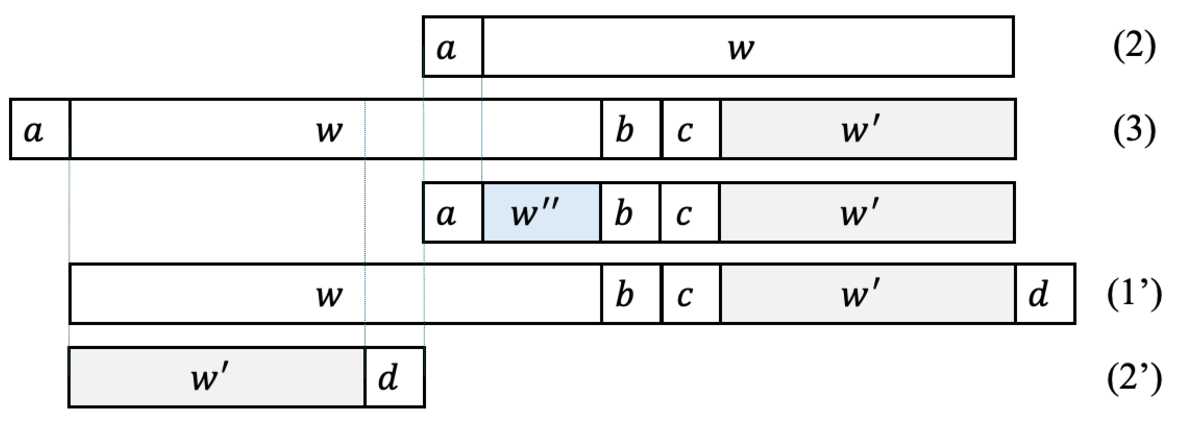
\includegraphics[scale=0.345]{figs/centerproof1.pdf}
      \caption{Case (a1) in Lemma~\ref{lem:addpart}: Relation of strings $w$, $w^{\prime}$, and $w^{\prime\prime}$}\label{fig:centerproof1}
    \end{center}
    \end{figure}

  Second, for the case (a2), we suppose that $(A, B) = (dy_{1}a, bc)$, i.e., $q = q_{1}dy_{1}awbcq_{2} $ holds.
  Then, the following conditions must be satisfied for $y_{1}^{\prime}\in X$:
  \begin{align*}
    \textrm{(1)}~& p_{1} \preceq q_{1}, & \textrm{(1')}~& p_{2} \preceq awbcq_{2}\mbox{ or} \\
    & & & p_{2} \preceq y_{1}^{\prime}awbcq_{2},\\
    \textrm{(2)}~& p_{1} \preceq q_{1}d\mbox{ or}  & \textrm{(2')}~& p_{2} \preceq wbcq_{2}, \\
    & p_{1} \preceq q_{1}dy_{1}^{\prime}, & & \\
    \textrm{(3)}~& p_{1} \preceq q_{1}dy_{1}aw, & \textrm{(3')}~& p_{2} \preceq q_{2}.
  \end{align*}
  %
  From $p_{1} \preceq q_{1}dy_{1}aw$ in (3), $p_{1}$ can be expressed as $p^{\prime}_{1}p^{\prime\prime}_{1}$ for some $p^{\prime}_{1}$ and $p^{\prime\prime}_{1}$, where $p^{\prime}_{1} \preceq q_{1}d$ and $p^{\prime\prime}_{1} \preceq y_{1}aw$.
  When $p_{2} \preceq awbcq_{2}$ in (1'), we have
  $$p=p^{\prime}_{1}p^{\prime\prime}_{1}xp_{2} \preceq q_{1}dp^{\prime\prime}_{1}xawbcq_{2}=q \{ y_{1}:=p^{\prime\prime}_{1}x \}.$$
  Thus, $p \{ x := xy \} \preceq q \{ y_{1}:=p^{\prime\prime}_{1}xy \}$ holds.
  This contradicts the assumption.
  When $p_{2} \preceq y_{1}^{\prime}awbcq_{2}$ in (1'), we similarly have
  $$p=p^{\prime}_{1}p^{\prime\prime}_{1}xp_{2} \preceq q_{1}dp^{\prime\prime}_{1}xy_{1}^{\prime}wbcq_{2}=q \{ y_{1}:=p^{\prime\prime}_{1}xy_{1}^{\prime} \}.$$
  Thus, $p \{ x := xy \} \preceq q \{ y_{1}:=p^{\prime\prime}_{1}xyy_{1}^{\prime} \}$ holds.
  This contradicts the assumption that $p \{ x := xy \} \not\preceq q$.
  %
  Similarly, we can show that the case $(A, B) = (bc, dy_{1}a)$ also contradicts the assumption.
  
  Finally, we prove that for the case (a3), $p \{ x := xy \} \preceq q$ holds. Suppose that $(A, B) = (y_{1}ay_{2}, bc)$, i.e., $q = q_{1}y_{1}ay_{2}wbcq_{2} $ holds. Then, the following conditions must be satisfied for $y_{1}^{\prime}\in X$:
  \begin{align*}
    \textrm{(1)}~& p_{1} \preceq q_{1}\mbox{ or} & \textrm{(1')}~& p_{2} \preceq y_{2}wbcq_{2}, \\
    & p_{1} \preceq q_{1}y_{1}^{\prime}, & & \\
    \textrm{(2)}~& p_{1} \preceq q_{1}dy_{1}, & \textrm{(2')}~& p_{2} \preceq wbcq_{2}\mbox{ or}\\    
    & & & p_{2} \preceq y_{2}^{\prime}wbcq_{2}, \\
    \textrm{(3)}~& p_{1} \preceq q_{1}y_{1}ay_{2}w, & \textrm{(3')}~& p_{2} \preceq q_{2}.
  \end{align*}
  %
  Let $q^{\prime}_{1}=q_{1}y_{1}a,~q^{\prime}_{2}=y_{2}w,~q^{\prime}_{3}=bcq_{2}$. From (3) and (1'), we have $p_{1} \preceq q^{\prime}_{1}q^{\prime}_{2}$ and $p_{2} \preceq q^{\prime}_{2}q^{\prime}_{3}$, respectively.
  Since $q_{2}^{\prime}$ contains a variable symbol, Theorem~\ref{Sato1:Lemma9} implies that $p \preceq q$ holds.
  This contradicts the assumption.
  %
  Similarly, we can show that the case $(A, B) = (bc, y_{1}ay_{2})$ also contradicts the assumption.
  
  \smallskip
  
  From the above, we conclude that if $p \{ x := r \} \preceq q$ for all $r = \{ ya, bc, dy \}$ (\TheConditionA), then $p \{ x := xy \} \preceq q$ holds.
  \end{proof}

  The condition in Lemma~\ref{lem:addpart} is illustrated in four cases (3)--(6) in Fig.~\ref{fig:lem5bigraph}.

  \begin{figure*}[t]
    \begin{center}
      \includegraphics[scale=0.525]{figs/lem5bigraph.pdf}
      \caption{Let $\Sigma=\{a,b,c,d,e,f,g\}$ and $p,q \in \RPat$. We assume that the symbols in $\Sigma$ are mutually distinct. The figure (3) expresses case $D = \{ ya, bc, dy \}$ in Lemma~\ref{lem:addpart}.
      The figures (4), (5), and (6) express three cases $D = \{ ya, bc, ay \}$, $D = \{ ya, bb, dy \}$, and $D = \{ ya, bb, ay \}$, respectively.
      In these cases, if $p \{ x := r \} \preceq q$ for all $r \in D$, then $p \{ x := xy \} \preceq q$ holds.}\label{fig:lem5bigraph}
    \end{center}
  \end{figure*}

% To position the next figure optimally in the paper, it is placed here. (by Takayoshi Shoudai)
\begin{figure*}[t]
  %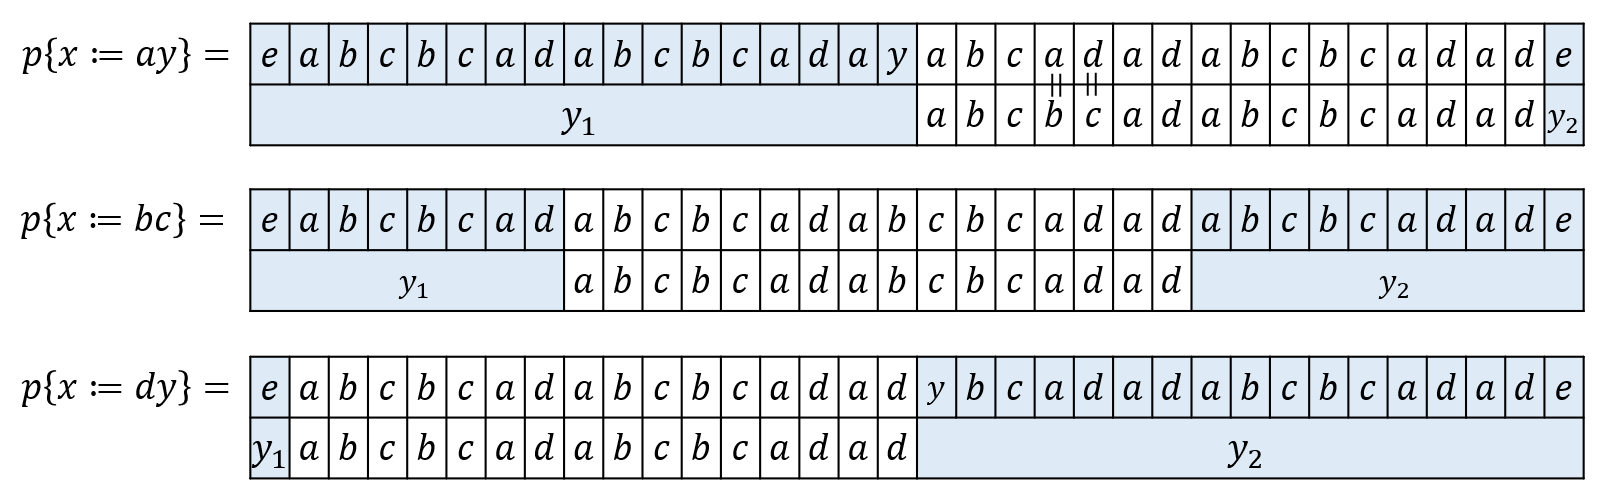
\includegraphics[width=\linewidth]{figs/Exam_b=a_c=d.png}
  \begin{center}
  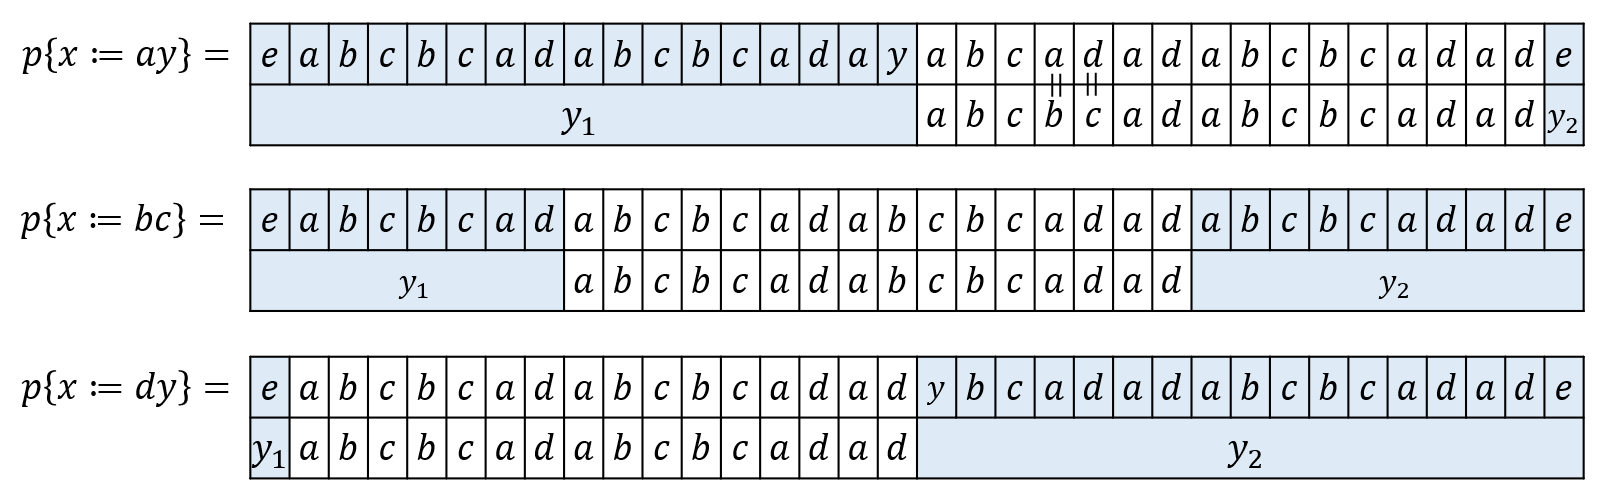
\includegraphics[scale=0.45]{figs/Exam_b=a_c=d.png}
  \end{center}
  \caption{Substitutions for $p$ and each correspondence to $q$.}
  \label{fig:cex-bacd}
\end{figure*}

\begin{lem}\label{lem:oneside}
Let $\Sigma$ be an alphabet with $\sharp\Sigma \ge 3$ and let $p,~q$ be regular patterns on $\Sigma\cup X$.
Let $D$ be one of the following sets of regular patterns on $\Sigma\cup X$, where $y$ is a variable symbol in $X$ that does not appear in $p$ and $q$.
\begin{enumerate}
\item[{\rm (i)}] $D=\{ ya, bc, dy \}$ (\TheConditionB),
\item[{\rm (ii)}] $D=\{ ya, bc, dy \}$ (\TheConditionC).
\end{enumerate}
Then, if $p \{ x := r \} \preceq q$ for all $r \in D$, it follows that $p \{ x := xy \} \preceq q$.
\end{lem}

In {\rm (i)}, we note that if $b = d$, then, because $p\{x:=dy\}\preceq q$, $p\{x:=bc\}\preceq q$ is always satisfied.
In this sense, $D$ essentially consists of only two elements.
To avoid this, we assume $b \not= d$.
In {\rm (ii)}, for the same reason, we assume $c\not= a$. 

\medskip

\begin{proof}
It is obvious if no variable symbol appears in $p$.
Therefore, let $p=p_{1}xp_{2}$, where $p_{i}$ (for $i=1,2$) is either the empty string or a regular pattern, and $x$ is a variable symbol.
We assume that $p \{ x := xy \} \not \preceq q$ in order to derive a contradiction.
In the case of \textrm{(ii)}, by reversing the strings $p$ and $q$, we can prove that the assumption $p \{ x := xy \} \preceq q$ leads to a contradiction, as in the case of \textrm{(i)}.
Therefore, in the following, we consider only the case of \textrm{(i)}: $D=\{ ya, bc, dy \}$ (\TheConditionB).

The proof is almost the same as the proof of Lemma~\ref{lem:addpart}.
Since $p \{ x := r \} \preceq q$ for all $r \in D$, there are three strings of length $2$ corresponding to $ya, bc, dy$ in $q$
The symbols appearing in $D$ correspond to either a variable or a constant symbol in $q$.
Let $y_{1}$ and $y_{2}$ be variable symbols appearing in $q$.
The strings $ya$ and $dy$ must correspond to the strings $y_{1}a$ and $dy_{2}$ in $q$, respectively.
For the same reasons stated at the beginning of Lemma~\ref{lem:addpart}, the string $bc$ corresponds to the string $bc$ in $q$ as well.
Let $A,B,C$ be regular patterns on $\Sigma \cup X$, where $\{ A,B,C \} = \{ y_{1}a,ac,dy_{3} \}$.
Since $p \{ x := xy \} \not \preceq q$, $q$ can be expressed in one of the following four forms:
Let $y_{1}, y_{2}$ be distinct variable symbols in $X$, and $q_{1}, q_{2}, w, w^{\prime}$ either the empty string or a regular pattern on $\Sigma\cup X$.
From the conditions $b = a$ and $b \not= d$, it follows that $a \not= d$.
\begin{enumerate}
\item[(i1)] $q=q_{1}AwBw^{\prime}Cq_{2}$, where $\{ A,B,C \} = \{ y_{1}a,ac,dy_{2} \}$.
\item[(i2)] $q=q_{1}AwBq_{2}$, where $\{ A,B \} = \{ y_{1}ac,dy_{2} \}$.
\item[(i3)] $q=q_{1}Aq_{2}$, where $A = dy_{1}ac$.
\end{enumerate}

In cases (i1) and (i2), similar to Lemma~\ref{lem:addpart}, it is shown that $q=q_{1}y_{1}awacw^{\prime}dy_{2}q_{2}$ and $q=q_{1}y_{1}acwdy_{2}q_{2}$, respectively, where $w$ and $w^{\prime}$ contain no variable symbols.

First, we consider case (i1).
For $q=q_{1}y_{1}awacw^{\prime}dy_{2}q_{2}$, the following conditions must be satisfied:
\begin{align*}
  \textrm{(1)}~& p_{1} \preceq q_{1}, & \textrm{(1')}~& p_{2} \preceq wacw^{\prime}dy_{2}q_{2}, \\
  \textrm{(2)}~& p_{1} \preceq q_{1}y_{1}aw, & \textrm{(2')}~& p_{2} \preceq w^{\prime}dy_{2}q_{2}, \\
  \textrm{(3)}~& p_{1} \preceq q_{1}y_{1}awacw^{\prime}, & \textrm{(3')}~& p_{2} \preceq q_{2}.
\end{align*}

From (1') and (2'), $wacw^{\prime}d$ and $w^{\prime}d$ are prefixes of $p_{2}$, and from (2) and (3), $awacw^{\prime}$ and $aw$ are suffixes of $p_{1}$.
  From these facts:
  \begin{itemize}
  \item $|w|=|w^{\prime}|$: $c = a$ holds.
  \item $|w|=|w^{\prime}|+1$: $w = w^{\prime}d = cw^{\prime}$ holds. Thus, from Proposition~\ref{prop:repstring_origin}, $c = d$ holds.
  \item $|w| = |w^{\prime}|+2$: $w = w^{\prime}da = acw^{\prime}$ holds. From Proposition~\ref{prop:repstring_base},  $c \in \{a, d\}$ holds.
  %Therefore, these cases contradict the condition \TheConditionBsub.
  \item $|w| \ge |w^{\prime}|+3$: From (2) and (3), there exists a string $w^{\prime\prime}$ of length $|w|-|w^{\prime}|-2$ such that $w=w^{\prime\prime}acw^{\prime}$ holds.
  Moreover, from (2) and (3), since $|aw| < |wacw^{\prime}|$ and $aw = aw^{\prime\prime}acw^{\prime}$, it follows that $aw^{\prime\prime}$ is a suffix of $w$.
  On the other hand, from (1') and (2'), $w^{\prime}d$ is a prefix of $w$.
  Since $|w^{\prime}d| + |aw^{\prime\prime}| = |w^{\prime}| + |w^{\prime\prime}| + 2 = |w|$, we have $w=w^{\prime}daw^{\prime\prime}$.
  Therefore, $w^{\prime}daw^{\prime\prime} = w^{\prime\prime}acw^{\prime}$ holds (Fig.~\ref{fig:centerproof2}).
  From Proposition~\ref{prop:repstring}, we have $c \in \{a, d\}$.
  \item $|w^{\prime}|=|w|+1$: From (1') and (2'), $c = d$ holds.
  \item $|w^{\prime}| = |w|+2$: From (1') and (2'), $d$ is a prefix of $w^{\prime}$. Thus, from (2) and (3), $w^{\prime} = wac = daw$ holds. From Proposition~\ref{prop:repstring_base}, $c \in \{a, d\}$ holds.
 \item $|w^{\prime}| \ge |w|+3$: From (1') and (2'), there exists a string $w^{\prime\prime}$ of length $|w|-|w^{\prime}|-2$ such that $w^{\prime}=wacw^{\prime\prime}$ holds.
  Moreover, from (1') and (2'), since $|w^{\prime}d| < |wacw^{\prime}|$ and $w^{\prime}d = wacw^{\prime\prime}d$, $w^{\prime}d$ is a prefix of $w^{\prime}$.
  On the other hand, from (1') and (2'), $aw^{\prime}w$ is a suffix of $w^{\prime}$.
  Since $|w^{\prime\prime}d| + |aw| = |w^{\prime}| + |w| + 2 = |w^{\prime}|$, we have $w^{\prime}=w^{\prime\prime}daw$.
  Therefore, $w^{\prime\prime}daw = wacw^{\prime\prime}$ holds.
  From Proposition~\ref{prop:repstring}, we have $c \in \{a, d\}$.
  %Therefore, these cases contradict the condition \TheConditionBsub.
  \end{itemize}
  All the cases contradict the condition \TheConditionBsub.
  Therefore, if \TheConditionB\ are satisfied, the case (i1) is impossible.

  \begin{figure}[t]
    \begin{center}
      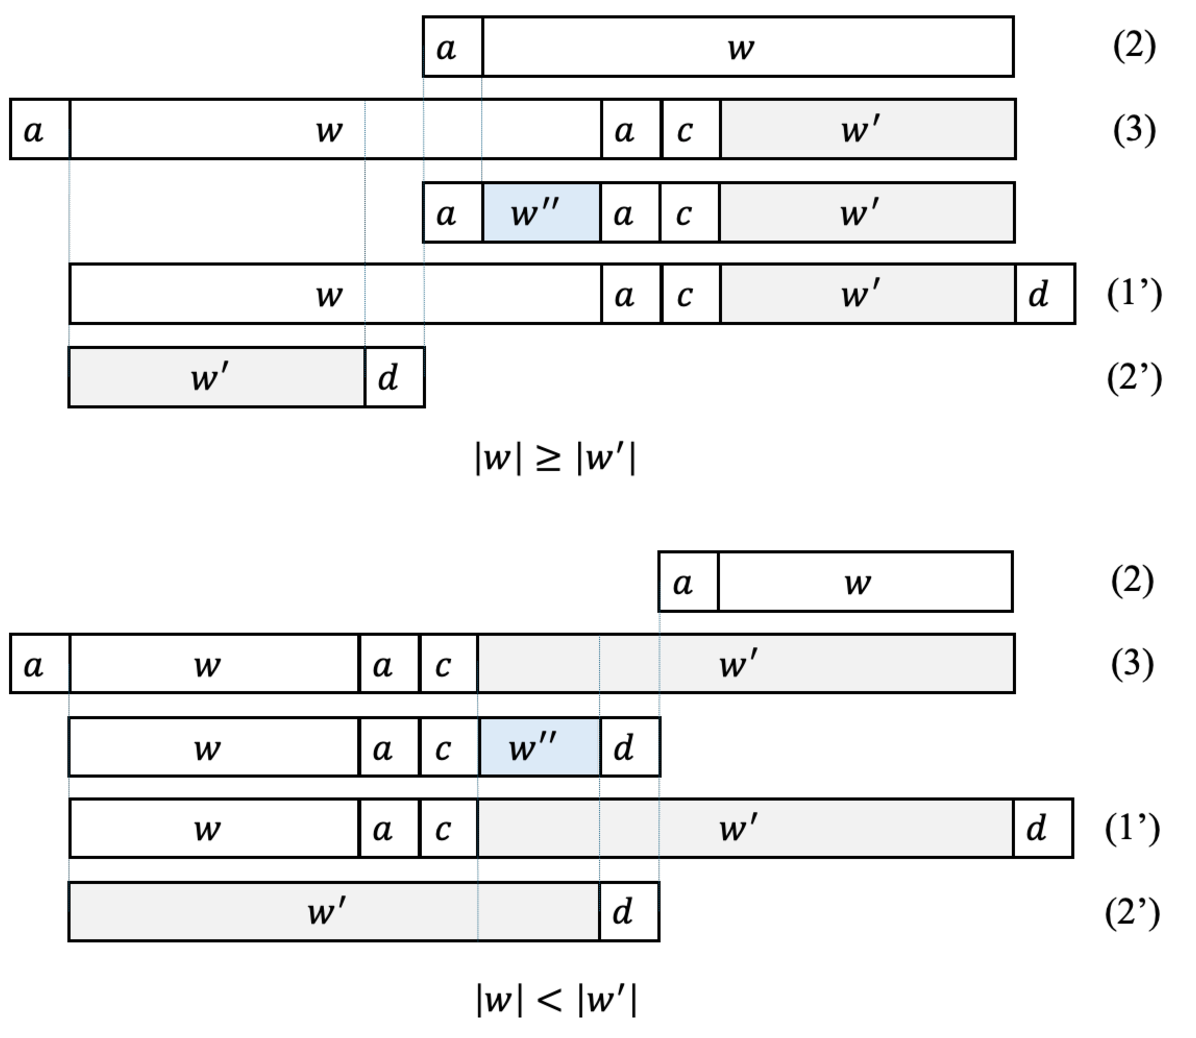
\includegraphics[scale=0.345]{figs/centerproof2.pdf}
      \caption{Case (i1) in Lemma~\ref{lem:oneside}: Relation of strings $w$, $w^{\prime}$, and $w^{\prime\prime}$}\label{fig:centerproof2}
    \end{center}
    \end{figure}

Second, we consider case (i2).
For $q=q_{1}y_{1}acwdy_{2}q_{2}$, the following conditions must be satisfied:
\begin{align*}
  \textrm{(1)}~& p_{1} \preceq q_{1}, & \textrm{(1')}~& p_{2} \preceq cwdy_{3}q_{2}, \\
  \textrm{(2)}~& p_{1} \preceq q_{1}y_{1}, & \textrm{(2')}~& p_{2} \preceq wdy_{3}q_{2}, \\
  \textrm{(3)}~& p_{1} \preceq q_{1}y_{1}acwdy_{3}, & \textrm{(3')}~& p_{2} \preceq q_{2}.
\end{align*}

\begin{itemize}
\item If $|w|=0$, from (1') and (2'), the prefix of $p_{2}$ is $cd$ and $d$. Thus, we have $c=d$.
\item If $|w|=1$, from (1') and (2'), the prefix of $p_{2}$ is $cwd$ and $wd$. Thus, we have $w=c=d$.
\item If $|w| \ge 2$, then from (1') and (2'), $cwd$ and $wd$ are prefixes of $p_{2}$. Thus, we have $cw=wd$. From Proposition~\ref{prop:repstring_base}, $c=d$ holds.
\end{itemize}
All of these cases do not meet \TheConditionB.
Therefore, if \TheConditionB\ are satisfied, the case (i2) is also impossible.

Finally, we consider case (i3).
For $q=q_{1}dy_{1}acq_{2}$, the following conditions must be satisfied for $y_{1}^{\prime},y_{1}^{\prime\prime}\in X$:
\begin{align*}
  \textrm{(1)}~& p_{1} \preceq q_{1}d \mbox{~or} & \textrm{(1')}~& p_{2} \preceq cq_{2}, \\
  &  p_{1} \preceq q_{1}dy_{1}^{\prime}, & & \\
  \textrm{(2)}~& p_{1} \preceq q_{1}dy_{1}, & \textrm{(2')}~& p_{2} \preceq q_{2}, \\
  \textrm{(3)}~& p_{1} \preceq q_{1}, & \textrm{(3')}~& p_{2} \preceq acq_{2} \mbox{~or}\\
  & & & p_{2} \preceq y_{1}^{\prime\prime}acq_{2}.
\end{align*}
For $p_{1} \preceq q_{1}d$ in (1) and $p_{2} \preceq acq_{2}$ in (3'), $p = p_{1}xp_{2} \preceq q_{1}dxacq_{2} \preceq q\{y_{1}:=x\}$ holds. From this, we have $p\{x:=xy\} \preceq q\{y_{1}:=x\}$. This contradicts the assumption that $p\{x:=xy\} \not\preceq q$. Similarly, we can show that the other cases of (1) and (3') also contradict the assumption.

From the above, we conclude that if $p \{ x := r \} \preceq q$ for all $r \in \{ ya, bc, dy \}$ (\TheConditionB), then $p \{ x := xy \} \preceq q$ holds.
\end{proof}

The conditions (i) and (ii) in Lemma~\ref{lem:oneside} are illustrated in the cases (7) and (8) in Fig.~\ref{fig:lem6bigraph}.

\begin{figure}[t]
  \begin{center}
    \includegraphics[scale=0.525]{figs/lem6bigraph.pdf}
    \caption{Let $\Sigma=\{a,b,c,d,e,f,g\}$ and $p,q \in \RPat$. We assume that the symbols in $\Sigma$ are mutually distinct.
    The figures (7) and (8) express two cases $D = \{ ya, ac, dy \}$ and $D = \{ ya, bd, dy \}$ in Lemma~\ref{lem:oneside}, respectively.
    In these cases, if $p \{ x := r \} \preceq q$ for all $r \in D$, then $p \{ x := xy \} \preceq q$ holds.}\label{fig:lem6bigraph}
  \end{center}
\end{figure}

When the conditions of both Lemmas \ref{lem:addpart} and \ref{lem:oneside} are not satisfied, counterexamples can be constructed as follows:

\begin{prop}\label{prop:bothsides}
  Let $\Sigma$ be an alphabet with $\sharp \Sigma \ge 3$.
  For a variable symbol $y$, let $D= \{ ya, bc, dy \}$ $(b = a$ and $c = d)$.
  There exist regular patterns $p$ and $q$ on $\Sigma\cup X$ such that $p \{ x := r \} \preceq q$ for any $r \in D$, but $p \{ x := xy \} \not \preceq q$.
\end{prop}

\begin{proof}
We provide an example to demonstrate this proposition.
Let $a,b,c,d,e$ be constant symbols in $\Sigma$, and let 
$x,y,y_{1},y_{2}$ be variable symbols in $X$.
Define the regular patterns $p$ and $q$ as follows:
\begin{align*}
p &= eabcbcadabcbcadaxbcadadabcbcadade,\\
q &= y_{1}abcbcadabcbcadady_{2}~~~~~(b = a\mbox{~and~}c = d).
\end{align*}

\noindent
Obviously $p \{ x:=xy \} \not \preceq q$ holds.
For these $p$ and $q$, the condition for Proposition~\ref{prop:bothsides} holds as follows (see also Fig.~\ref{fig:cex-bacd}):
\begin{eqnarray*}
&p& \{ x:=ya \} \\ 
& = & (eabcbcadabcbcaday)abcadadabcbcadade\\
& = & q \{ y_{1} := eabcbcadabcbcaday,~y_{2}:=e \} \\
& \preceq & q,\\
&p& \{ x:=bc \}  \\
& = & (eabcbcad)abcbcadabcbcadad(abcbcadade) \\
& = & q \{ y_{1} := eabcbcad,~y_{2} := abcbcadade \} \\
& \preceq & q,\\
&p& \{ x:=dy \}  \\
& = & eabcbcadabcbcadad(ybcadadabcbcadade) \\
& = & q \{ y_{1}:=e,~y_{2} := ybcadadabcbcadade \} \\
& \preceq & q.
\end{eqnarray*}
\end{proof}

%\hfill Edited by Takayoshi Shoudai
%\hrule
%\bigskip